A good definition for Monte Carlo methods is given by Malvin H. Kalos and Paula A. Whitlock in Ref\cite{MonteCarloMethods}:
\begin{center}
  \quote\textit{A definition of a Monte Carlo method would be one that involves deliberate use of random numbers in a calculation that has the structure of a stochastic process.}
\end{center}

We should then clarify that a Monte Carlo method is not a simulation of a stochastic process but uses a stochastic process to solve non-probabilistic problems.
Another important note we need to make, sice we are going to use computers to deploy these methods, is that machines cannot generate true-random numbers. What computers do with functions like \texttt{rand()} in \texttt{C} is to generate a sequence of numbers that maintain all the properties of random numbers, thus we may call them pseudo-random numbers.

\section{Monte Carlo evaluation of integrals}

Many computational problems involve the evaluation of integrals and in the majority of them the integration space is multidimensional.
For example in classical mechanics we may want to simulate a gas in thermal equilibrium using the canonical ensemble.
The problem reduces to the computation of the integral

\begin{equation}
  \expval{ E } = \dfrac{ \int \mc{H}(\vec{r},\vec{p})e^{-\beta\mc{H}(\vec{r},\vec{p})} d^{3N}\vec{r}d^{3N}\vec{p} }{ \int e^{-\beta\mc{H}(\vec{r},\vec{p})} d^{3N}\vec{r}d^{3N}\vec{p} }.
  \label{canonical}
\end{equation}

To simulate a gas with a decent approximation to reality you cannot use less than 100 particles and even in this case you have to deal with two 600-dimensional integrals.
Noticing that the kinetic part is given analytically we are still left with 300-dimensional integrals.
Calculating this integrals with traditional methods (e.g. Simpson) requires evaluating the integrand at each point of a regular quadrature.
To achieve for example $10\%$ of relative error for the integral you would need to calculate the integrand on something around $10^D$ points, where $D$ is the space dimension.
Even if your computer could handle $10^{15}$ calculations of integrands per second and you only consider 20 particles ($D=60$) you would need $10^{45}$ seconds, while the age of the universe is $10^{34}$ seconds.
These are the kind of problems where Monte Carlo methods suits perfectly.

The Monte Carlo integration is based on the Central Limit theorem, which states that given $x_1,\dots,x_N$ independent and identically distributed stochastic variables, if N is sufficiently large, the expectation value of $\expval{ f(x)}=\int \mc{P}(x) f(x)dx$ can be approximated with its mean value $S_N=\frac{1}{N}\displaystyle\sum_{i=1}^{N}f(x_i)$:

\begin{equation}
  \lim_{N \to \infty}S_N=\expval{ f(x)}.
\end{equation}

Furthermore If $N$ is finite, yet large, the theorem tells us that the probability distribution function of the mean value is a Gaussian with $FWHM=\sigma_N=\sqrt{\frac{1}{N}\expval{ (f-\expval{ f})^2}}$:

\begin{equation}
  \mc{P}(S_N)=\frac{1}{\sqrt{2\pi \sigma_N^2}}e^{-\frac{(S_N-\expval{ f})^2}{2\sigma_N^2}}.
\end{equation}

$\sigma_N$ represent the statistical error and it relates to the variance through the formula

\begin{equation}
  \sigma_N=\sqrt{\frac{1}{N}(\expval{f^2}-\expval{f}^2)}.
  \label{staterror}
\end{equation}

This means that we can tackle integrals as the one in \autoref{canonical} with a reasonable computation time by generating random variables distributed with the probability density function

\begin{equation}
  \mc{P}(x)=\dfrac{ e^{-\beta V(\vec{r})} }{ \int e^{-\beta V(\vec{r})} d^{3N}\vec{r} }.
\end{equation}

A question now arises spontaneously: How can I generate variables with a custom probability density function?

\section{Markov chains and Metropolis algorithm}

\newcommand{\T}[2]{T_{#1}\left(\bm{R}_{#2}\leftarrow \bm{R}_{#1}\right)}
An effective method for sampling with custom probability is using the so-called Markov chains, that is essentially another way of referring to a random walk.
Lets say that at time zero our system has coordinates $\bm{R}_0$ sampled from an arbitrary distribution $\mc{P}_0(\bm{R}_0)$.
We then define a transition matrix $\T{i}{i+1}$ that represent the probability density of finding the system in $\bm{R}_{i+1}$ after it was in $\bm{R}_i$. Therefore

\begin{equation}
  \mc{P}_1=\int d\bm{R}_0 \mc{P}_0(\bm{R}_0)\T{0}{1}=\hat{T}_0\mc{P}_0(\bm{R}_0)
\end{equation}

Where we introduced the integral operator $\hat{T}_i =\int d\bm{R}_i \mc{P}_i(\bm{R}_i)\T{i}{i+1}$.
Iterating the chain we find

\begin{equation}
  \mc{P}_i(\bm{R}_i)=\hat{T}_{i-1}\mc{P}_{i-1}(\bm{R}_{i-1})=\hat{T}_{i-1}\dots\hat{T}_0\mc{P}_0
\end{equation}

\begin{figure}
  \centering
  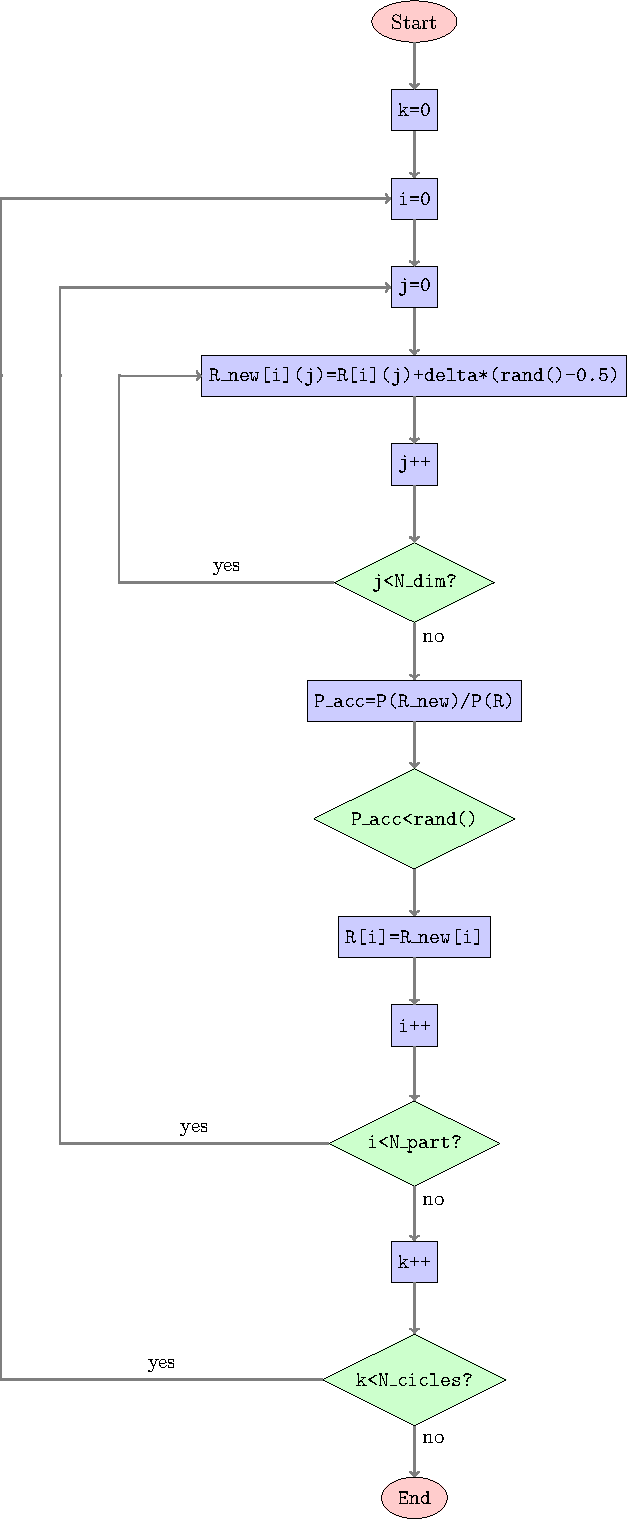
\includegraphics[width=.6\textwidth]{Schemes/metropolis.pdf}
  \caption[Metropolis algorithm scheme.]{Metropolis algorithm scheme. Notice that \texttt{rand()} is supposed to generate uniform distributed random numbers in$(0,1]$.}
  \label{Metropolis}
\end{figure}

For our purposes we are only interested in stationary chains, namely $\hat{T}_j=\hat{T}\forall j$, so that the probability at step $i$ depends only on the transition matrix and $\mc{P}_0$.
Now lets suppose that our chain is convergent, and hence $\lim_{i\to\infty}=\mc{P}_{\infty}$, or in other words $\mc{P}_{\infty}$ is an eigenvector of $\hat{T}$ with eigenvalue 1 (otherwise we would loose the normalization property of $\mc{P}_{\infty}$).
This means that if we iterate the chain from $\bm{R}_0$ with a transition matrix having such properties, after a sufficient amount of steps, say $k$, we will obtain a chain where every element is distributed with the probability density $\mc{P}_{\infty}$.
Therefore calling $m$ the total number of steps of the random walk, thanks to the Central Limit theorem, we can compute the expected value of our quantity $f$ as

\begin{equation}
  \dfrac{1}{m-k}\sum_{i=k+1}^m f(\bm{R}_i)
\end{equation}

An easy way of defining a transition matrix with the properties described above is given by the Metropolis algorithm. The full derivation can be found in Ref\cite{Pederiva2017} or more detailed in Ref\cite{MonteCarloMethods}.
Here I will only show a flow chart in \autoref{Metropolis}.

At each iteration the algorithm generates a new configuration moving the coordinates of the particles randomly within a box of side$\Delta$.
Anyway it is convenient to consider new configurations also when only one particle coordinates change.
Then it calculates the acceptance probability, defined as
\begin{equation}
  \mc{P}_{acc}=\min\left(1,\dfrac{\mc{P}(\bm{R}_{new})}{\mc{P}(\bm{R})}\right)
  \label{Pacc}
\end{equation}
where $\mc{P}=\mc{P}_{\infty}$ is the probability that we want to sample.
This ratio represent the probability of accepting the transition.
In order to follow this probability, when choosing if discard or accept the move, we can generate a uniform distributed random variable and accept when $\mc{P}_{acc}$ is smaller or discard otherwise.

\subsection{The correlation problem}
\label{correlation}

One of the hypothesis of the Central Limit theorem was that the variables need to be independent.
Unfortunately variables generated with Markov chains are not independent, since every configuration depends on the previous one.
If we use the Metropolis algorithm the key parameter that determines how much two neighbour configurations are correlated is the length $\Delta$.
If $\Delta$ is too large than new configurations are more likely to be discarded since they can easily move away from the equilibrium, while if it is too small configurations will be too similar.
In both cases we obtain high correlation.
One has to calibrate the parameter $\Delta$ in order to reduce correlation to a minimum.
Even if we choose $\Delta$ to minimize correlation two neighbour samples will always be correlated, so we are left with 2 possibilities: taking ``void" steps or blocking.
The first means to compute the desired quantities every, say, $\tau$ time steps, so that for $\tau$ sufficiently large samples will be almost independent.
The correlation of the samples can then be calculated as

\begin{equation}
  \bar{C}_{\tau}(f)=\dfrac{\expval{ f(\bm{R}_i)f(\bm{R}_{i+\tau})}-{\expval{ f}}^2}{\expval{ f^2}-{\expval{ f}}^2}.
\end{equation}

$C_{\tau}(f)$ usually has an exponential decay $C_{\tau}(f)\sim e^{-\frac{i}{\tau}}$,so that the true error can be approximated as $\sigma_N^2\tau$.

For blocking we mean that we calculate the average of the quantity for $N_{block}$ time steps, and then we treat these mean values as our independent data samples.
In this way the overall average will not change but the variance will be (about) the correct one.

Accurate calculation of $\Delta$ to minimize correlation is really expensive in terms of computation time and requires additional programming.
A simple effective rule is to keep the acceptance ratio $\dfrac{accepted}{total}$ between $30\%$ and $50\%$ and use a conservative blocking\cite{Pederiva2017}.
I tried to keep acceptance around $40\%$ and blocking every $1000$ time steps.

\section{Quantum Variational Monte Carlo}

A recurrent problem in quantum mechanics is to calculate the eigenvalue of an observable:

\begin{equation}
  \hat{O}\ket{\Psi_k}=O_k\ket{\Psi_k}
\end{equation}

Unfortunately the analytical solution of this equations is rarely available and we have to use some numerical method instead.
For some cases we can use exact diagonalization techniques, but usually the computational cost increases exponentially with the number of particles.
On the other hand a large variety of Monte Carlo methods has been developed in order to solve this kind of problems and we usually refer to these methods as Quantum Monte Carlo methods (QMC).

In particular, if we want to find the ground state, the simplest method, but still largely used because of his effectiveness and interpretability, is the Variational Monte Carlo and as the name suggests it makes use of the variational principle:

\begin{equation}
  E_0\leq E[\Psi_T]=\dfrac{\expval{\Psi_T|\mc{H}|\Psi_T}}{\expval{\Psi_T|\Psi_T}}=\dfrac{\int \Psi_T^*(\bm{R})\mc{H}(\bm{R})\Psi_T(\bm{R})d\bm{R}}{\int \sqmod{\Psi_T(\bm{R})}d\bm{R}}.
\end{equation}

The principle means that given a trial wave function $\Psi_T$ the energy associated will be always greater or at most equal than the actual ground state.
The idea is to write a realistic trial wave function including some parameters ${\bm{\alpha}}$ so that we can minimize the energy as a function of those parameters.
The variational principle in terms of the parameters would read

\begin{equation}
  E_0\leq E({\bm{\alpha}})=\dfrac{\int \Psi_T^*(\bm{R};{\bm{\alpha}})\mc{H}(\bm{R})\Psi_T(\bm{R};{\bm{\alpha}})d\bm{R}}{\int \sqmod{\Psi_T(\bm{R};{\bm{\alpha}})}d\bm{R}}.
\end{equation}

At this point we might wonder if we can use some Monte Carlo integration method to solve the integral above, and indeed, just by a simple manipulation, we can rewrite it in the desired form:

\begin{equation}
  \int \mc{P}(\bm{R};\bm{\alpha})E_{loc}(\bm{R};\bm{\alpha})d\bm{R}
\end{equation}

Having defined the local energy as

\begin{equation}
  E_{loc}(\bm{R};\bm{\alpha})=\dfrac{\mc{H}\Psi_T(\bm{R};\bm{\alpha})}{\Psi_T(\bm{R};\bm{\alpha})}
  \label{Eloc}
\end{equation}

And the probability is given by

\begin{equation}
  \mc{P}(\bm{R};\bm{\alpha})=\dfrac{\sqmod{\Psi_T(\bm{R};\bm{\alpha})}}{\int \sqmod{\Psi_T(\bm{R};{\bm{\alpha}})}d\bm{R}}.
  \label{Qprob}
\end{equation}

The problem is now reduced to find the minimum in the parameters space of $E(\bm{\alpha})$.
It is important to notice though that the variational principle does not ensure that the minum we find in this we will be equal to the actual ground state.
If we want our minimum to be as close as possible to $E_0$ we need to use a realistic trial wave function.
